\documentclass[conference]{IEEEtran}
\IEEEoverridecommandlockouts

\usepackage{cite}
\usepackage{amsmath,amssymb,amsfonts}
\usepackage{graphicx}
\usepackage{textcomp}
\usepackage[table]{xcolor}
\usepackage{float}
\usepackage{subfig}
\usepackage{booktabs}
\usepackage{svg}
\usepackage{verbatim}
\usepackage{algorithm}
\usepackage{algpseudocode}

\begin{document}

\title{Design and Implementation of Tracking Filters for a Passive Radar System}

\author{\IEEEauthorblockN{Itumeleng Malemela\textsuperscript{1,2},
Stephen Paine\textsuperscript{1},
Francois Schonken\textsuperscript{1}}
\IEEEauthorblockA{\textsuperscript{1}Department of Electrical Engineering, University of Cape Town, South Africa\\
\textsuperscript{2}Council for Scientific and Industrial Research (CSIR), South Africa\\
\{mlmitu002, stephen.paine, francois.schonken\}@uct.ac.za, imalemela@csir.co.za}
}

\maketitle

\begin{abstract}
Passive Radar exploits existing transmitter infrastructure to detect targets through their skin returns. FM Passive Radar offers high Doppler resolution due to longer integration times but faces challenges including clutter, direct and multipath interference, and low range resolution due to limited bandwidth. While tracking filters have been widely studied, their application to commercial aircraft tracking using FM signals in the bistatic range-Doppler domain remains limited. This paper presents the design and evaluation of four tracking filters, namely the Kalman, Unscented Kalman, Particle, and Recursive Gauss-Newton filters, incorporating an adaptive covariance scaling mechanism to handle outliers and zero-Doppler cancellation artefacts. A processing chain comprising DPI cancellation, CA-CFAR detection, and mean-shift clustering is implemented to provide measurements for tracking. Filters are assessed through log-likelihood benchmarks, corroborated by RMSE and NIS consistency, computational load, and data association metrics using the Flexible Extensible Radar Simulator across multiple flight scenarios. The Recursive Gauss-Newton Filter achieves the best log-likelihood performance while meeting real-time constraints.
\end{abstract}

\begin{IEEEkeywords}
adaptive filters, FM Passive Radar, Kalman filters, Recursive Gauss-Newton filter, Particle filter, log likelihood, radar tracking filters, multi-target tracking
\end{IEEEkeywords}

\section{Introduction}

Ever since the emergence of Radio Detection and Ranging (Radar) technology, there has been a tremendous evolution in Radar systems. Modern Radar systems are now capable of not only detecting and determining range but also tracking, identifying, and classifying targets in cluttered environments \cite{Richards2010}. Passive Radar (PR) systems detect and track objects by passively receiving and analysing signals from external sources, known as illuminators of opportunity, including Frequency Modulation (FM) radio, DVB-T, and cellular broadcasts \cite{Howland2005a}. This characteristic allows PR systems to operate without emitting any signals, making them advantageous for covert operations and cost-effective applications.

FM radio is considered one of the most capable high-powered illuminators of opportunity for long-range PR detection \cite{De2015}, offering widespread availability, weather robustness, and no spectrum licensing requirements. Although its low bandwidth yields poor range resolution, these attributes make FM PR attractive for cost-effective air traffic control at small airports in developing countries.

Specifically, this work designs and evaluates four tracking filters for commercial aircraft tracking in the bistatic range and Doppler domain using FM PR, incorporating an adaptive covariance scaling mechanism and a log-likelihood (LL) based performance assessment among other metrics such as the Root Mean Square Error (RMSE), Normalised Innovation Squared (NIS), and computational load across simulated flight scenarios. The paper also evaluates the data association performance of the Multi-Target Tracking (MTT) framework across different false alarm probabilities.

\section{System Overview}

The simulation framework comprises four key stages: the Radar environment, modelled using the Flexible Extensible Radar Simulator (FERS); the Radar processing chain; the tracking filters; and the MTT system, as depicted in Fig.~\ref{fig:radarOverview}.

\begin{figure}[H]
    \centering
    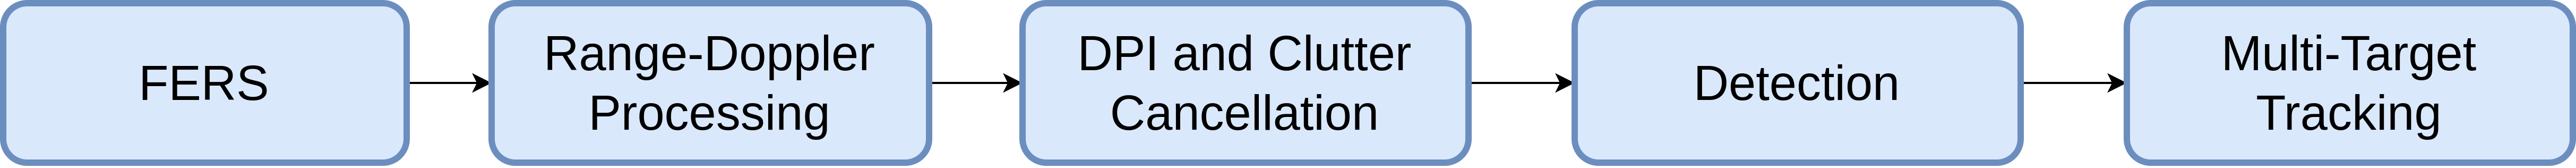
\includegraphics[width=1\linewidth]{figures/radarOverview.drawio.png}
    \caption{Radar system overview.}
    \label{fig:radarOverview}
\end{figure}

\subsection{Flexible Extensible Radar Simulator}

FERS \cite{fersMarc} is used to simulate a bistatic Radar configuration with one transmitter, two receivers (reference and surveillance), and targets, as illustrated in Fig.~\ref{fig:360_3D}. The transmitter is modelled as an isotropic FM illuminator at 94~MHz, the receivers use directional antennas, and the transmitter-receiver baseline is 12.5~km.

\subsection{Radar Processing Chain}

From the FERS output files, the reference and surveillance signals are reconstructed into complex baseband form. The Amplitude Range Doppler (ARD) map is computed in discrete time as:
\begin{equation}
  \left| \Psi(\tau, v) \right| = \left| \sum_{n=0}^{N-1} s_E(n) s_R^*(n-\tau) e^{j 2\pi v n/N} \right|
\end{equation}
where $\Psi(\tau, v)$ is the ARD map, $s_E(n)$ represents the echo signal, and $s_R^*(n-\tau)$ is the complex conjugate of the reference signal. Range-Doppler processing utilizes 200 kilosamples per second. Fig.~\ref{fig:ardMap} illustrates the resulting ARD map, where the dominant peak at zero bistatic Doppler corresponds to Direct Path Interference (DPI) leakage into the surveillance channel, with additional peaks at similar ranges arising from sidelobes of the FM waveform's ambiguity function. Although the cross-correlation function enhances processing gains, it also amplifies DPI and clutter which is undesired, leading to side-lobes that mask target returns.

\begin{figure}[t]
  \centering
  \includesvg[width=0.85\linewidth,inkscapelatex=false]{figures/ardMapFinal.svg}
  \caption{Amplitude/Range/Doppler map.}
  \label{fig:ardMap}
\end{figure}


\subsubsection{DPI and Clutter Suppression}

To improve detection performance, DPI and clutter are suppressed from the surveillance channel prior to range-Doppler processing. The Extensive Cancellation Algorithm (ECA), based on the least mean squares estimator, is applied due to its fast convergence and demonstrated effectiveness in clutter suppression \cite{coloneECA}. Cardinali \textit{et al.}\ demonstrated the superior performance of the ECA in achieving nearly complete clutter suppression in \cite{cardinali2007comparison, Heunis2010}.

\subsubsection{Target Detection}

Each cell in the range-Doppler map is evaluated against an adaptive threshold using a Cell Averaging Constant False Alarm Rate (CA-CFAR) detector \cite{Shrivathsa2008a}, which allows tuning of the detection probability through the probability of false alarm $P_{fa}$. The noise power $P_n$ from training cells is scaled by a factor $\alpha$ to determine the detection threshold:
\begin{equation}
  T = \alpha \cdot P_n, \quad \alpha = N \cdot (P_{fa}^{-1/N} - 1),
\end{equation}
where $N$ is the number of training cells \cite{Sambath2020a}. Because the target spans multiple range bins due to the limited bandwidth of the FM waveform, averaging is applied only in the Doppler domain, where higher resolution is available. The CA-CFAR uses 4 guard cells and 6 training cells on each side, with $P_{fa} = 10^{-5}$ selected through sensitivity analysis as shown in Fig.~\ref{fig:cfarValidation}.

\begin{figure}[t]
  \centering
  \includesvg[width=0.85\linewidth,inkscapelatex=false]{figures/ca_cfar_validate_corrections_v2.svg}
  \caption{CA-CFAR threshold at 15\,km bistatic range for $P_{fa}$ values from $10^{-3}$ to $10^{-7}$ at simulation time $t = 2$\,s.}
  \label{fig:cfarValidation}
\end{figure}

\subsubsection{Target Centroiding}
\label{subsec:centroiding}

The CFAR output produces multiple detections across adjacent Doppler and range cells. To generate measurements suitable for tracking, these detections are grouped into clusters using mean-shift clustering, which does not require prior knowledge of the number of targets and directly provides cluster centroids \cite{cheng1995mean, derpanis2005mean}. The bandwidths used are 5~Hz and 10~km for the Doppler and range dimensions, respectively. Fig.~\ref{fig:cfar_centroids} shows the CFAR output with the extracted centroids.

\begin{figure}[t]
  \centering
  \includesvg[width=0.7\linewidth,inkscapelatex=false]{figures/cacfar_pfa7_centroid_correction.svg}
  \caption{CA-CFAR output with mean-shift clustering centroids at simulation time $t = 2$\,s.}
  \label{fig:cfar_centroids}
\end{figure}

\section{Tracking Filters and Adaptive Filtering}

\subsection{Doppler Range Target Tracking}

The centroids obtained from clustering provide estimates of the target's position in the bistatic range-Doppler domain. To track the target state, a Nearly Constant Velocity (NCV) model is adopted, suitable for non-manoeuvring targets such as commercial aircraft \cite{Li2003a}. The NCV state vector is defined as:
\begin{equation}
  x(t) = [r_t, \dot{r_t}, f_t, \dot{f_t}]^T,
\end{equation}
where $r_t$ and $f_t$ denote bistatic range and Doppler, and $\dot{r_t}, \dot{f_t}$ their rates. The discrete time evolution is
\begin{equation}
  \mathbf{X}_k =
  \begin{bmatrix}
      1 & \tau & 0 & 0 \\
      0 & 1 & 0 & 0 \\
      0 & 0 & 1 & \tau \\
      0 & 0 & 0 & 1
  \end{bmatrix} X_{k-1} + w_{k-1},
\end{equation}
with sampling interval $\tau$ and zero mean Gaussian process noise $w_{k-1}$ whose covariance is:
\begin{equation}
  Q = S_w
  \begin{bmatrix}
      \tfrac{\tau^4}{4} & \tfrac{\tau^3}{2} & 0 & 0 \\
      \tfrac{\tau^3}{2} & \tau^2 & 0 & 0 \\
      0 & 0 & \tfrac{\tau^4}{4} & \tfrac{\tau^3}{2} \\
      0 & 0 & \tfrac{\tau^3}{2} & \tau^2
  \end{bmatrix},
\end{equation}
where $S_w$ denotes the process noise spectral density, applied per-axis as $S_{w,r}$ and $S_{w,\dot{r}}$ for the range and Doppler blocks, respectively \cite{Measurements2023b}.

\subsection{Tracking Filters Overview}

The Kalman Filter (KF) provides the linear Gaussian baseline and is valued for its computational efficiency and robustness \cite{Julier1997a}. The Unscented Kalman Filter (UKF) uses the unscented transform to propagate sigma points through non-linear functions without requiring Jacobians \cite{Julier1997a}. The Particle Filter (PF) uses Monte Carlo methods to represent the posterior distribution, with systematic resampling to mitigate particle degeneracy, offering a robust alternative when both the system dynamics and noise are highly non-linear and non-Gaussian \cite{Arulampalam2007, NJGordon}. The Recursive Gauss-Newton Filter (RGNF) aims to improve numerical performance and adaptivity to unknown dynamics, and has demonstrated effectiveness in both non-linear tracking scenarios and linear cases such as Doppler-only and bistatic Radar tracking \cite{Inggs1, De2015, roaldje}.


\subsection{Log Likelihood}
The LL is used as the primary statistical benchmark to evaluate each filter's performance. Unlike the RMSE, which measures trajectory error independently of the filter covariance, and the NIS\footnote{Under a Gaussian innovation assumption, $e_k^T S_k^{-1} e_k$ follows a $\chi^2$ distribution with $n$ degrees of freedom, so mean NIS values close to $n$ (the measurement dimension) indicate a well-calibrated innovation covariance.}, which validates the calibration of the innovation covariance \cite{BarShalom2001}, the LL jointly captures estimation accuracy and filter uncertainty through the error covariance matrix $\mathbf{P}$ \cite{labbe2014kalman, Grewal2006}. The LL at time step $k$ is defined as:
\begin{equation}
  \ell_k = -\frac{1}{2}\left[\ln|S_k| + e_k^T S_k^{-1} e_k + n\ln(2\pi)\right],
\end{equation}
where $S_k = H_k P_k^- H_k^T + R_k$ is the innovation covariance, $e_k = z_k - H_k \hat{X}_k^-$ is the innovation, and $n$ is the dimension of the measurement vector; higher (less negative) values of $\ell_k$ indicate better statistical consistency between the filter estimates and the ground truth.


% =============================================================
% Reviewer requests addressed in this subsection:
%   R1(1)  "complete pseudocode"                       -> Algorithm 1
%   R1(1)  "the forgetting factor alpha"               -> alpha=0.98 (closing paragraph)
%   R1(1)  "initial Q/R settings"                      -> Table filter_params
%   R1(1)  "positive-definiteness safeguards"          -> convex-combination sentence
%   R1(1)  "unified tuning protocol for all filters"   -> "same update rules...all four filters"
%   R2(1)  "how Q is updated"                          -> Q equation (Akhlaghi Eq. 15) + PF analogue
%   R2(1)  "when covariance scaling is triggered"      -> continuous; outliers handled at MTT gate
%   R2(1)  "value of forgetting factor alpha"          -> alpha=0.98 stated
%   R2(1)  "initial R/Q setting"                       -> Table filter_params
%   R2(1)  "criteria for judging innovation anomalies" -> deferred to MTT chi-squared gate
%   R2(1)  "consistent across the four filters"        -> closing paragraph with PF analogue
%
% Preamble additions required (once):
%   \usepackage{algorithm}
%   \usepackage{algpseudocode}
% =============================================================

\subsection{Adaptive Filtering}

Accurate state estimation depends on the appropriate selection of the measurement noise covariance $\mathbf{R}$ and process noise covariance $\mathbf{Q}$. Fixed values of these matrices may degrade tracking performance under
deviations from the assumed motion model or in the presence of outliers, which is particularly relevant in the tracking of commercial aircraft to achieve stable and smooth trajectory estimates. Adaptive filtering addresses this limitation by adjusting $\mathbf{R}$ and $\mathbf{Q}$ during operation \cite{Mehra1972}. Among several
approaches, covariance matching is adopted in this work.

The covariance scaling method updates $\mathbf{R}$ and $\mathbf{Q}$ using the innovation and residual, defined as:

\begin{equation}
d_k = z_k - h_k(\hat{X}^-_k), \quad \varepsilon_k = z_k - h_k(\hat{X}^+_k),
\end{equation}

where $z_k$ is the measurement, and $\hat{X}^-_k, \hat{X}^+_k$ are the predicted and estimated states respectively. For adaptive estimation of $\mathbf{R}$, the innovation covariance is:

\begin{equation}
S_k = H_k P^-_k H_k^T + R_k,
\end{equation}

leading to the update:

\begin{equation}
R_k = \alpha R_{k-1} + (1-\alpha)(\varepsilon_k \varepsilon_k^T + H_k P^-_k H_k^T),
\end{equation}

where $0 \leq \alpha \leq 1$ is a forgetting factor \cite{Akhlaghi2018}. The process-noise covariance is adapted analogously using the residual-based rule of \cite{Akhlaghi2018}:

\begin{equation}
Q_k = \alpha Q_{k-1} + (1-\alpha)\,(K_k\, d_k d_k^T\, K_k^T),
\end{equation}

where $K_k$ is the Kalman gain. Both updates are convex combinations of positive semi definite matrices, preserving the positive-definiteness of $\mathbf{R}_k$ and $\mathbf{Q}_k$.

\begin{algorithm}[t]
\caption{Adaptive Covariance Scaling (per scan $k$)}
\label{alg:covscaling}
\begin{algorithmic}[1]
    \State Compute $d_k$, $S_k$, $K_k$ from the filter's native prediction and update.
    \State Compute the post-update residual $\varepsilon_k \gets z_k - h_k(\hat{X}^+_k)$.
    \State $R_k \gets \alpha R_{k-1} + (1-\alpha)(\varepsilon_k \varepsilon_k^T + H_k P^-_k H_k^T)$
    \State $Q_k \gets \alpha Q_{k-1} + (1-\alpha)(K_k d_k d_k^T K_k^T)$
    \end{algorithmic}
\end{algorithm}

Since the Q update presumes an explicit Kalman gain, step 4 of Algorithm~\ref{alg:covscaling} is applied only in the KF, UKF and RGNF, while steps 1--3 apply to all four filters. Algorithm~\ref{alg:covscaling} runs on every accepted measurement rather than being triggered by an innovation-anomaly criterion; outliers are rejected upstream by the Mahalanobis gate (Section~\ref{sec:mtt}), so the updates operate only on accepted measurements. In the PF, the empirical particle-cloud covariance replaces $H_k \mathbf{P}^-_k H_k^T$ in the R update, and $\mathbf{Q}$ is used at prediction but not adapted online. Nominal values shared across all four filters are seeded from measurement-chain resolution and target dynamics under the bistatic geometry. The measurement noise covariance is $\mathbf{R}_0 = \operatorname{diag}(1.0,\,0.25)$, set from the FM range resolution and Doppler cluster bandwidth. The process noise covariance $\mathbf{Q}_0$ follows Eq.~(5) with spectral densities $S_{w,r} = 0.1$ and $S_{w,\dot{r}} = 0.02$, reflecting the commercial aircraft acceleration envelope projected through the bistatic range-rate mapping. The initial state covariance is $\mathbf{P}_0 = \operatorname{diag}(5, 1, 2, 1)$, and the forgetting factor is $\alpha = 0.98$.

\subsection{Multi-Target Tracking}
\label{sec:mtt}

The implemented MTT framework consists of gating, Global Nearest Neighbour (GNN) association, and an M-out-of-N track management strategy. Gating rejects unlikely detection-to-track associations using an ellipsoidal validation region based on the Mahalanobis distance \cite{Jerrelind2020, Richards2010}:
\begin{equation}
  Z_k S_k^{-1} Z_k^T \leq G,
\end{equation}
where $G$ is the gating threshold. Observations within the gate are assigned using the GNN method, which minimizes the distance measure \cite{Konstantinova2003}:
\begin{equation}
  d^2_{G_{ij}} = d^2_{ij} + \ln|S_i|.
\end{equation}
Unassigned detections are used to initiate new tracks. Track confirmation is based on the M-out-of-N rule, in which a track is promoted from tentative to confirmed if a detection is observed in at least $M$ of the last $N$ scans.

\section{Simulations and Results}

\begin{figure*}[t]
\centering
\subfloat[]{%
  \includesvg[width=0.38\linewidth,inkscapelatex=false]{figures/3D_360.svg}%
  \label{fig:360_3D}%
}%
~
\subfloat[]{%
  \includesvg[width=0.38\linewidth,inkscapelatex=false]{figures/360_filter_output.svg}%
  \label{fig:360FilterOutputs}%
}%
\\[2.6mm]
\caption{360\textdegree{} orbit manoeuvre scenario: (a) bistatic Radar geometry in the FERS simulation showing Tx, SurvRx, and RefRx positions with the target trajectory in Cartesian coordinates; (b) tracking filter predictions, measurements, and ground truth in the bistatic range and Doppler domain.}
\label{fig:360_scenario}
\end{figure*}

The tracking filters are evaluated across three FERS flight scenarios representing common commercial aircraft manoeuvres in the bistatic range and Doppler domain: a take-off manoeuvre (60~s), a landing manoeuvre with descent and turn (120~s), and a 360\textdegree{} orbit (120~s).

\subsection{360\textdegree{} Orbit Manoeuvre}

The 360\textdegree{} orbit manoeuvre, illustrated in Fig.~\ref{fig:360_scenario}(a), represents a common holding pattern for commercial aircraft at constant altitude. The closed-loop bistatic range and Doppler trajectory in Fig.~\ref{fig:360_scenario}(b) presents a challenging scenario due to continuous rate changes in both domains. All four filters successfully track the target through the full orbit, with the RGNF and KF maintaining the most stable LL. Range predictions show a slight offset from ground truth, as measurement covariance is configured with lower range sensitivity to mitigate FM bandwidth-induced fluctuations.



% =============================================================
% Reviewer requests addressed in this subsection:
%   R1(2)  "actual LL values, means, variances"           -> Table filter_perf reports mean +/- std across N_MC FERS runs
%   R1(2)  "error bars / confidence intervals"            -> Table filter_perf mean +/- std format
%   R1(2)  "clarify the ranking criterion"                -> replaced ranks with actual metric values
%   R2(2)  "add RMSE / MAE trajectory-error metrics"      -> RMSE rows in Table filter_perf
%   R2(2)  "add NIS consistency test"                     -> Mean NIS row in Table filter_perf + interpretation
%   R2(2)  "discuss how covariance scaling biases LL"     -> Section III.C (Tracking Performance Metrics) + RMSE corroboration here
%   R2(3)  "scenario naming consistency"                  -> take-off / landing / 360 orbit used throughout
% =============================================================

\subsection{Tracking Performance Evaluation}
The LL is the primary metric, with RMSE (covariance-independent) and NIS (covariance-calibration) as cross-checks, since adaptive $\mathbf{R}$/$\mathbf{Q}$ updates can improve LL through covariance calibration without necessarily reducing trajectory error. All metrics are mean~$\pm$~standard deviation across $N_{\mathrm{MC}}$ FERS-seeded MC runs.

\begin{figure}[t]
  \centering
  \includesvg[width=0.7\linewidth,inkscapelatex=false]{figures/360_doppler_ll.svg}
  \caption{Doppler LL for the 360\textdegree{} orbit manoeuvre scenario.}
  \label{fig:dopplerLogLike360}
\end{figure}

Fig.~\ref{fig:dopplerLogLike360} shows the Doppler LL for the 360\textdegree{} orbit scenario. The RGNF maintains the most stable values throughout, while the UKF exhibits significant dips during turns as its sigma-point spread amplifies the effect of corrupted Doppler measurements. The KF and PF show consistent behaviour, though the PF produces a lower overall LL due to the variance inherent in particle-based estimation. Table~\ref{tab:filter_perf} presents the mean LL, RMSE and NIS across all three flight scenarios.

\begin{table}[t]
\centering
\caption{Filter performance across scenarios (mean~$\pm$~standard deviation over 100 Monte Carlo runs with FERS, with the first 10 scans of each run excluded to remove filter-initialisation transient). LL and NIS are averaged per scan, and RMSE is computed over the same window; RMSE units are km (range) and Hz (Doppler); higher LL and lower RMSE are better; mean NIS target is $2$. \textbf{Bold} indicates best per row.}
\label{tab:filter_perf}
\setlength{\tabcolsep}{2pt}
\scriptsize
\begin{tabular*}{\columnwidth}{@{\extracolsep{\fill}}llcccc@{}}
\toprule
\textbf{Scen.} & \textbf{Metric} & \textbf{KF} & \textbf{UKF} & \textbf{RGNF} & \textbf{PF} \\
\midrule
Landing & LL$_r$        & $-1.68{\pm}0.03$ & $\mathbf{-1.67{\pm}0.03}$ & $-1.71{\pm}0.03$ & $-3.10{\pm}0.25$ \\
        & LL$_{\dot r}$ & $\mathbf{-1.91{\pm}0.02}$ & $-2.28{\pm}0.01$ & $-2.05{\pm}0.01$ & $-3.46{\pm}0.09$ \\
        & RMSE$_r$      & $1.37{\pm}0.07$ & $\mathbf{1.24{\pm}0.08}$ & $\mathbf{1.24{\pm}0.07}$ & $3.45{\pm}3.80$ \\
        & RMSE$_{\dot r}$ & $2.21{\pm}0.01$ & $\mathbf{2.17{\pm}0.01}$ & $\mathbf{2.17{\pm}0.01}$ & $4.84{\pm}10.95$ \\
        & NIS           & $\mathbf{0.99{\pm}0.03}$ & $0.91{\pm}0.03$ & $0.95{\pm}0.03$ & $0.26{\pm}0.33$ \\
\addlinespace
360\textdegree{} Orbit & LL$_r$        & $-1.69{\pm}0.07$ & $-1.68{\pm}0.07$ & $\mathbf{-1.60{\pm}0.05}$ & $-2.85{\pm}0.02$ \\
      & LL$_{\dot r}$ & $-3.42{\pm}0.54$ & $-3.64{\pm}3.07$ & $\mathbf{-2.65{\pm}0.06}$ & $-4.24{\pm}0.07$ \\
      & RMSE$_r$      & $1.12{\pm}0.14$ & $1.16{\pm}1.02$ & $\mathbf{1.05{\pm}0.13}$ & $1.16{\pm}0.27$ \\
      & RMSE$_{\dot r}$ & $4.17{\pm}0.31$ & $4.58{\pm}5.03$ & $\mathbf{3.54{\pm}0.99}$ & $4.78{\pm}2.75$ \\
      & NIS           & $2.66{\pm}0.21$ & $\mathbf{2.21{\pm}0.18}$ & $2.74{\pm}0.10$ & $0.21{\pm}0.08$ \\
\addlinespace
Take-off & LL$_r$        & $-1.77{\pm}0.14$ & $-1.78{\pm}0.17$ & $\mathbf{-1.71{\pm}0.14}$ & $-3.21{\pm}0.04$ \\
         & LL$_{\dot r}$ & $-1.82{\pm}0.04$ & $-2.10{\pm}0.02$ & $\mathbf{-1.81{\pm}0.02}$ & $-3.34{\pm}0.16$ \\
         & RMSE$_r$      & $\mathbf{1.47{\pm}0.29}$ & $1.51{\pm}0.24$ & $1.51{\pm}0.24$ & $2.55{\pm}3.40$ \\
         & RMSE$_{\dot r}$ & $\mathbf{1.20{\pm}0.02}$ & $1.32{\pm}0.03$ & $1.27{\pm}0.02$ & $4.66{\pm}13.41$ \\
         & NIS           & $\mathbf{0.87{\pm}0.15}$ & $0.81{\pm}0.18$ & $0.84{\pm}0.19$ & $0.11{\pm}0.24$ \\
\bottomrule
\end{tabular*}
\end{table}

The LL results show the RGNF outperforming the other filters on the 360\textdegree{} orbit and take-off scenarios in both range and Doppler, while on the landing scenario the LL differences are marginal ($\leq0.14$), with the UKF leading in range and the KF in Doppler. The RMSE cross-check confirms this ranking on the 360\textdegree{} orbit, where the RGNF achieves the lowest range and Doppler RMSE (1.05~km and 3.54~Hz); on take-off the KF is marginally lower on both axes, while on landing the RGNF ties with the UKF for the lowest RMSE. NIS calibration is closest to the target of~2 on the challenging 360\textdegree{} orbit scenario, where the UKF is best-calibrated at 2.21, followed by the KF at 2.66 and the RGNF at 2.74, whereas the landing and take-off NIS values sit below~1, reflecting a conservatively-sized innovation covariance during near-linear segments. The PF ranks last or near-last across LL and RMSE because the bistatic problem is near-linear-Gaussian and the KF, UKF and RGNF handle it near-optimally, so the PF's sample-based posterior adds Monte Carlo variance without benefit.

\subsection{Computational Load}
% ---------------------------------------------------------------
% Paragraph 1 -- experimental setup.
% Addresses R1 bullets: hardware/software disclosure, implementation
% language/libraries, and reproducible timing settings.
% ---------------------------------------------------------------
The computational load of each filter was evaluated on a Dell Precision
7550 workstation (Intel Core i9-10885H, 32~GB RAM) running Gentoo Linux
(kernel 6.18.38), with all filters implemented in MATLAB R2025a and
executed single-threaded. To isolate intrinsic filter cost from shared
multi-target tracking overhead (gating, GNN association, and track
management), each filter's prediction and update stages were driven
directly with the sequence of clustered centroids from
Section~\ref{subsec:centroiding} and timed with the \texttt{tic} and
\texttt{toc} functions, averaged over 1\,000 Monte Carlo runs of a 60~s
single-target scenario after a 10-scan warm-up.


% ---------------------------------------------------------------
% Table II — raw per-scan filter cost, absolute μs + ratio.
% Addresses R1: absolute runtimes (not just ratios) and variability
% on Monte Carlo timing. Values are the mean and standard deviation
% of per-run averages across the 1000 MC runs.
% ---------------------------------------------------------------
\begin{table}[t]
    \centering
    \caption{Per-scan runtime of each tracking filter (mean~$\pm$~standard deviation across 1\,000 MC runs). Ratios are relative to KF.}
    \label{tab:comp_load}
    \begin{tabular*}{\columnwidth}{@{\extracolsep{\fill}}lcccc@{}}
        \toprule
        & \multicolumn{2}{c}{\textbf{Update} ($\mu$s)} & \multicolumn{2}{c}{\textbf{Predict} ($\mu$s)} \\
        \cmidrule(lr){2-3} \cmidrule(lr){4-5}
        \textbf{Filter} & $\mu \pm \sigma$ & Ratio & $\mu \pm \sigma$ & Ratio \\
        \midrule
        KF   &   29.1~$\pm$~11.0  & 1.00  &   22.0~$\pm$~7.9   & 1.00 \\
        RGNF &   51.0~$\pm$~20.8  & 1.75  &   32.5~$\pm$~12.7  & 1.47 \\
        UKF  &  121.6~$\pm$~44.0  & 4.18  &  146.6~$\pm$~57.6  & 6.66 \\
        PF   & 1619.0~$\pm$~570.4 & 55.71 & 1703.1~$\pm$~648.8 & 77.31 \\
        \bottomrule
    \end{tabular*}
\end{table}
  

% ---------------------------------------------------------------
% Paragraph 2 — interpretation of raw filter costs.
% REWRITTEN to match new ratios; the previous "UKF slightly faster
% update / heavier predict" story no longer applies.
The RGNF's update and prediction stages cost 1.5 to 1.8 times the KF
baseline, arising from iterative Gauss-Newton refinement that converges
within a small number of iterations for the range-Doppler measurement
model. The UKF's stages cost 4 to 7 times the baseline, reflecting
propagation of $2n{+}1 = 9$ sigma points through the state model. The
PF's stages exceed the baseline by nearly two orders of magnitude,
driven by $N = 10\,000$ particle propagation, likelihood evaluation,
and systematic resampling.




% ---------------------------------------------------------------
% Paragraph 3 -- MTT scaling, wraps around Fig. mtt_output.
% ---------------------------------------------------------------
In an MTT framework, each confirmed track runs an independent filter
instance, so per-scan cost is expected to grow linearly with the number
of confirmed tracks $N_t$. Because each filter's innovation covariance
$S_k$ drives the gating and GNN association behaviour, wider or more
variable $S_k$ can in principle produce additional phantom tracks and
cause per-scan cost to grow faster than $N_t$.

\begin{figure}[htbp]
  \centering
  \includesvg[width=0.85\linewidth,inkscapelatex=false]{figures/mtt_3_tracking_corrections_v1.svg}
  \caption{MTT output using a KF with GNN association and 3-out-of-4 M-out-of-N track management for a
three-target scenario.}
  \label{fig:mtt_output}
\end{figure}

Table~\ref{tab:comp_scaling} reports the measured MTT-inclusive per-scan
cost at $N \in \{1,3,5,10\}$ target scenarios. Empirically, cost grows
sub-linearly with confirmed track count: an increase in $N_t$ by a
factor of 8.4 between the $N{=}1$ and $N{=}10$ scenarios yields a
per-scan cost increase of only a factor of 2.5 to 3.1 across the four
filters, indicating that the fixed MTT overhead from gating, GNN
association, and track management inflates the per-scan computational
budget above the raw per-track filter work in this
regime~\cite{Konstantinova2003}. The PF's 29.9~ms per scan at
$N{=}10$ remains more than an order of magnitude below the 0.5--1~s
coherent processing interval typical of FM PR~\cite{Howland2005a};
the KF and RGNF stay below 2.5~ms per scan at $N{=}10$, offering the
most favourable computational profile for MTT deployment.


% ---------------------------------------------------------------
% Table III -- Measured MTT-inclusive per-scan cost vs N.
% ---------------------------------------------------------------
\begin{table}[t]
\centering
\caption{Measured MTT-inclusive per-scan cost ($\mu$s, mean~$\pm$~standard deviation) versus number of target scenarios
$N$. Mean confirmed track counts observed at each scenario are 1.0, 2.7, 5.0, and 8.4, respectively.}
\label{tab:comp_scaling}
\begin{tabular*}{\columnwidth}{@{\extracolsep{\fill}}lcccc@{}}
  \toprule
  \textbf{Filter} & $N{=}1$ & $N{=}3$ & $N{=}5$ & $N{=}10$ \\
  \midrule
  KF   &   945~$\pm$~72   &  1023~$\pm$~92   &  1566~$\pm$~107  &  2376~$\pm$~153  \\
  RGNF &   808~$\pm$~35   &   928~$\pm$~66   &  1424~$\pm$~73   &  2207~$\pm$~124  \\
  UKF  &  1383~$\pm$~57   &  1591~$\pm$~67   &  2527~$\pm$~80   &  3867~$\pm$~199  \\
  PF   &  9585~$\pm$~462  & 11696~$\pm$~515  & 19014~$\pm$~649  & 29858~$\pm$~1697 \\
  \bottomrule
\end{tabular*}
\end{table}
  


% =============================================================
% Reviewer requests addressed in this subsection:
%   R1(3)  "statistical meaning of Tables III-V"          -> captions state MC methodology and metric semantics
%   R1(3)  "define whether values are single-run / mean / total / normalized"
%                                                         -> captions clarify metric is a count per MC run summary
%   R1(3)  "evaluation window / normalization method"    -> methodology paragraph specifies 1000 MC runs and 3-target scenario
%   R1(3)  "report mean +/- variability"                 -> Tables V-VII to be extended to mean +/- std after MC re-run
% =============================================================

\subsection{Data Association Performance}

MTT data association is evaluated using true track confirmation (TTC), false track confirmation (FTC), and true track deletion (TTD) metrics, following \cite{kennedy2014powerful}. TTC counts true targets ever held by a confirmed track, FTC counts confirmed tracks with no true-target association, and TTD counts true targets whose track was deleted at any point. Filter covariance shapes both the gating threshold and the nearest-neighbour choice, so each filter yields a different GNN behaviour. Metrics are averaged over 100 FERS-seeded Monte Carlo runs of a three-target scenario (60~s at 1~s scan interval) at each CFAR $P_{fa}$ value.

\begin{table}[t]
    \centering
    \caption{Multi-target track management performance across CFAR $P_{fa}$ values (mean $\pm$ standard deviation over 100 Monte Carlo runs of the three-target scenario). \textbf{Bold} indicates best per row.}
    \label{tab:mtt_data_assoc}
    \scriptsize
    \setlength{\tabcolsep}{2pt}
    \begin{tabular*}{\columnwidth}{@{\extracolsep{\fill}}lcccc@{}}
        \toprule
        $\mathbf{P_{fa}}$ & \textbf{KF} & \textbf{UKF} & \textbf{RGNF} & \textbf{PF} \\
        \midrule
        \multicolumn{5}{@{}l}{\textit{True track confirmations}} \\
        $10^{-5}$ & 2.86${\pm}$0.35 & $\mathbf{3.00{\pm}0.00}$ & $\mathbf{3.00{\pm}0.00}$ & $\mathbf{3.00{\pm}0.00}$ \\
        $10^{-7}$ & 2.86${\pm}$0.35 & $\mathbf{3.00{\pm}0.00}$ & 2.99${\pm}$0.10 & $\mathbf{3.00{\pm}0.00}$ \\
        $10^{-9}$ & 2.86${\pm}$0.35 & $\mathbf{3.00{\pm}0.00}$ & $\mathbf{3.00{\pm}0.00}$ & $\mathbf{3.00{\pm}0.00}$ \\
        \addlinespace
        \multicolumn{5}{@{}l}{\textit{False track confirmations}} \\
        $10^{-5}$ & 3.58${\pm}$0.79 & 3.60${\pm}$0.72 & $\mathbf{3.54{\pm}0.70}$ & 4.23${\pm}$0.76 \\
        $10^{-7}$ & 2.97${\pm}$0.87 & 2.94${\pm}$0.87 & 2.92${\pm}$0.82 & $\mathbf{2.48{\pm}0.78}$ \\
        $10^{-9}$ & $\mathbf{1.86{\pm}0.78}$ & 2.02${\pm}$0.86 & 2.04${\pm}$0.62 & 2.03${\pm}$0.80 \\
        \addlinespace
        \multicolumn{5}{@{}l}{\textit{True track deletions}} \\
        $10^{-5}$ & 1.03${\pm}$0.17 & $\mathbf{1.00{\pm}0.00}$ & 1.08${\pm}$0.27 & 1.54${\pm}$0.50 \\
        $10^{-7}$ & 1.05${\pm}$0.22 & $\mathbf{1.00{\pm}0.00}$ & 1.01${\pm}$0.10 & 1.27${\pm}$0.45 \\
        $10^{-9}$ & 1.02${\pm}$0.10 & $\mathbf{1.00{\pm}0.00}$ & $\mathbf{1.00{\pm}0.00}$ & 1.26${\pm}$0.44 \\
        \bottomrule
    \end{tabular*}
\end{table}

Table~\ref{tab:mtt_data_assoc} shows the UKF, RGNF, and PF confirm all three targets on nearly every run, while the KF occasionally fails to confirm the farthest target, as its narrower innovation gate under-associates the sparser detections from weaker signal returns. False track confirmations decrease monotonically as $P_{fa}$ tightens; the PF is the outlier, producing the most at $P_{fa}{=}10^{-5}$ and the fewest at $10^{-7}$. The UKF's tight sigma-point $S_k$ yields the most stable track IDs across all $P_{fa}$, whereas the PF is the least stable due to particle-cloud dispersion fragmenting tracks into competing IDs.

\section{Conclusion}

This paper presented four tracking filters, namely the KF, UKF, PF, and RGNF, for FM PR commercial aircraft tracking in the bistatic range-Doppler domain, incorporating adaptive covariance scaling to mitigate outliers from zero-Doppler cancellation and FM bandwidth limitations. A complete processing chain comprising ECA-based DPI cancellation, CA-CFAR detection with sensitivity-tuned $P_{fa}$, and mean-shift clustering was implemented to provide measurements for tracking.

Among the four tracking filters evaluated, the RGNF is the most effective choice for FM PR commercial aircraft tracking. It delivers the highest log-likelihood on the demanding 360\textdegree{} orbit and take-off scenarios and the lowest orbit RMSE at only $1.75{\times}$ the KF runtime, establishing it as a practical baseline for real-time FM PR tracking. The KF remains a valid low-cost alternative on near-linear trajectories such as landing, while the PF adds Monte Carlo variance without benefit on this predominantly linear-Gaussian problem.

Future work includes validating with real-world PR system data, extending the tracking framework to the Interacting Multiple Model (IMM) approach for improved handling of manoeuvring commercial aircraft, exploring deep learning methods for complex target dynamics, investigating Multiple Hypothesis Tracking for improved data association, and optimization techniques for tracking filter parameter tuning.

\bibliographystyle{IEEEtran}
\bibliography{IEEEabrv,references}

\end{document}
